\chapter{Lo stato attuale}
\thispagestyle{empty}
\section{Le modifiche al giorno d'oggi}
%Aggiungi un mini indice in questo capitolo se le dimensioni dello stesso iniziano ad essere proibitive.\\
%Parla anche dell'assenza di organi per la misurazione dei consumi (elettrici e termici) e quindi problemi per la valutazione energetica \emph{ante-operam} e per il rispetto ai requisiti \emph{CAM}.\vspace{1em}
Nel primo capitolo si sono descritti in maniera sommaria l'architettura, l'edilizia e gli impianti presenti nell'intero complesso ospedaliero (al momento della costruzione) riportando le parole dell'\tit{ing.}{Corrado Beguinot}. In questo capitolo, invece, si vuole dare ampio spazio alle condizioni attuali del suddetto edificio, riportando i dati di input inseriti all'interno dello studio pre-riqualificazione energetica riferiti, quindi, allo stato di fatto. 

Prima di procedere con suddetto elenco particolareggiato sull'edificio 2, però, si vogliono riportare le modifiche effettuate su tutto l'impianto ospedaliero del policlinico. 

In questi anni, infatti, nella centrale termica, le caldaie vengono fatte funzionare per inviare acqua calda nella rete di teleriscaldamento non più a \n{170}{\degreeCelsius} ma a \n{130}{\degreeCelsius}. Per quanto riguarda il teleriscaldamento.
Il cogeneratore è stato modicato. Sono stati aggiunti questi gruppi frigoriferi di cui tot ad assorbimento.
\clearpage
\section{L'edificio 2}
Tutto il corpo di fabbrica è destinato alla \emph{Cardiochirurgia}.

Esso è costituito da 5 edifici:
\begin{itemize}
	\item Corpo A: è l'edificio principale. Di sviluppo longitudinale lungo un asse orientato lungo la direttrice N-E -- S-O, è alto 5 piani oltre il piano terra. Contiene le degenze, gli ambulatori, l'Emodinamica al piano terra, l'UTIC (Unità di Terapia Intensiva Coronarica) e il blocco operatorio al quinto piano. La sua superficie in pianta è di ... per un totale di ... per i 6 piani.
	\item Corpo B: contiene ... di pianta quadrata ed è alto solo 1 piano. Estensione
	\item Corpo C: contiene laboratori e ambulatori. E' di pianta rettangolare e alto solo 1 piano. Estensione
	\item Corpo D: contiene ... di pianta quadrata ed è alto solo 1 piano. Estensione
	\item Corpo E: contiene ... di pianta quadrata ed è alto solo 1 piano. Estensione
\end{itemize}

I livelli dell'edificio 2 (che sono comunque in comune con quasi tutti gli edifici del Policlinico) sono 8 di cui 2 sotterranei. Infatti, è presente una rete di cunicoli al di sotto del Policlinico che unisce in modo diretto e senza ostacoli (in quanto non è permesso il traffico veicolare al pubblico) i vari edifici. I livelli dei cunicoli sono due: uno è quello \emph{del pulito} (-1) mentre l'altro è quello \emph{dello sporco} (-2).

\textbf{Questa parte mettila dopo aver parlato dell'involucro opaco e trasparente}
Il suddetto edificio è stato suddiviso per questioni di comodità e calcolo in \emph{5~strutture}:
\begin{itemize}
	\item l'\emph{UTIC} è presente al primo piano dell'edificio alto. Comprende le sale operatorie e le relative degenze.
	\item \emph{Emodinamica} situata al piano terra dell'edificio alto. Comprende la sala operatoria, una sala operatoria minore e le relative sale controllo.
	\item il \emph{Quinto Piano} dell'edificio alto. Qui è presente la \emph{Terapia Intensiva}.
	\item il \emph{Corpo Alto} coincide con l'edificio alto escluse le 3 suddette strutture già menzionate. Sono presenti le degenze, le cucine, i servizi e gli uffici.
	\item il \emph{Corpo Basso} collegato a quello alto tramite un doppio tunnel di cui solo uno è oggetto di studio: sono presenti i laboratori di \emph{Patologia Immunitaria}.
\end{itemize}
Si riporta in Fig.~\vref{planimetriapianoterra} la planimetria del Piano Terra con i contorni colorati che evidenziano le zone di intervento. %Ricorda di dire prima perchè ci sono zone di intervento
\begin{sidewaysfigure}
	\centering
	\caption{Planimetria del Piano Terra dell'Edificio 2. Si notino le due aree di intervento.}
	\label{planimetriapianoterra}
	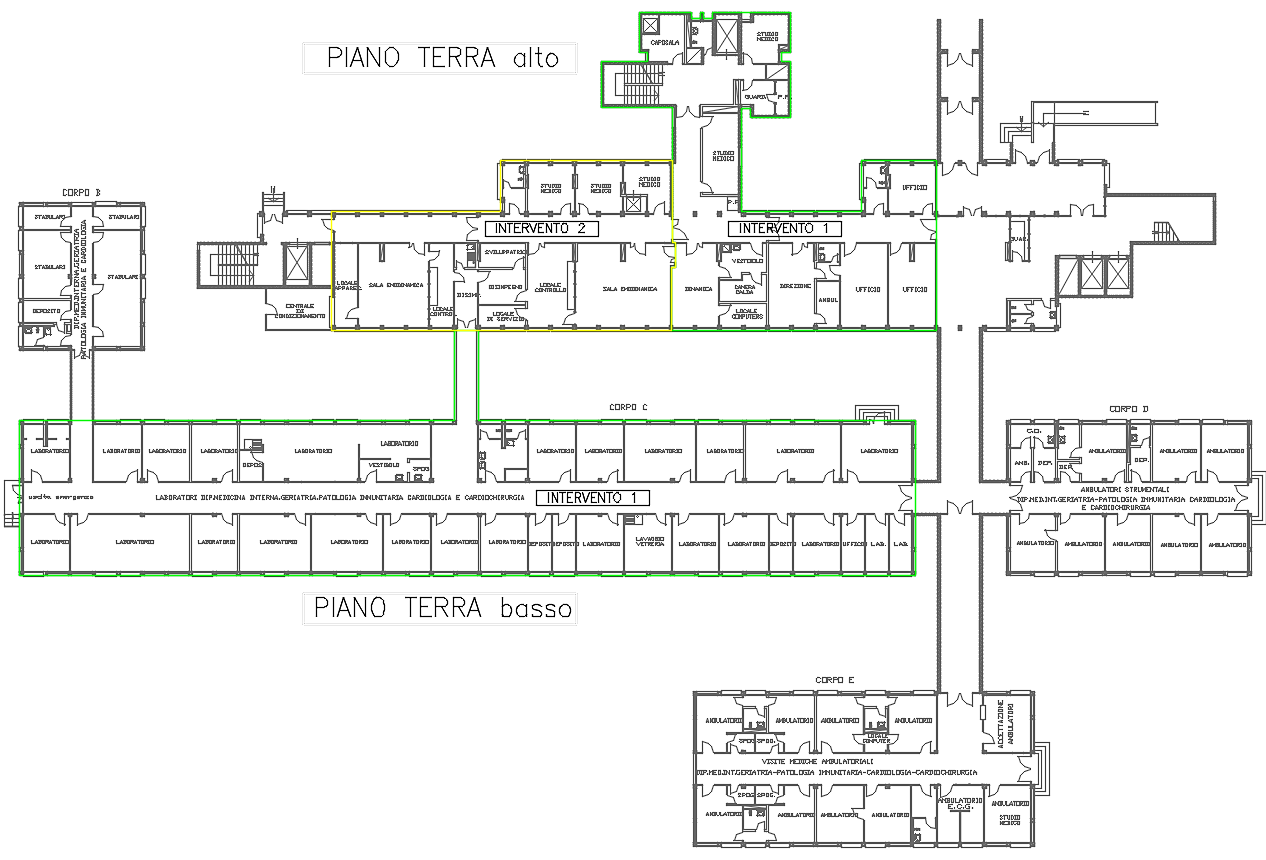
\includegraphics[width=\textheight]{6_2_cap/img/piano_terra}	
\end{sidewaysfigure}

L'edificio 2 preserva tutte le opere edili e impiantistiche realizzate all'epoca della sua costruzione. Non è difficile dedurre, quindi, che allo stato attuale sia i comportamenti estivi e invernali dell'involucro come le efficienze termo-meccaniche dell'impianto idro-aeraulico siano quantomeno inferiori a quelli consigliati dalla norma attuale vigente. 

%\begin{itemize}
%	\item componenti opachi
%	\item componenti trasparenti
%	\item ponti termici???
%	\item definizione dei vari locali
%\end{itemize}
%Metti i risultati con tabelle. 
%Inserisci foto in bianco e nero di alcuni componenti finestrati o criticità.
%Prendi in considerazione l'idea di inserire planimetrie da stampare su A3 da piegare all'interno della tesi. 
\section{L'involucro}
L'involucro dell'Edificio 2, sia quello opaco che quello trasparente, non è cambiato in questi anni quindi non ci sono differenze con le stratigrafie indicate dall'\tit{Ing.}{Corrado Beguinot}.

Si passa ora a descrivere i componenti (opachi e trasparenti) utilizzati come dati di input per il calcolo del fabbisogno energetico e del carico termico (estivo e invernale) dell'edificio stesso.
\subsection{Componenti opachi}
\subsubsection{MURO EXT}
È il componente esterno delle facciate maggiori del Corpo A. \\È caratterizzato esternamente da blocchi di silicalcite alternati dagli infissi. \\Questa tipologia di muro è fittizia poiché si è modellato un componente che nella realtà è caratterizzata da una diversa stratigrafia in senso verticale. Dal punto di vista numerico, quindi, si è effettuata una media ponderale delle varie caratteristiche termo-fisiche in modo tale che il risultato finale sia quanto più possibile veritiero. La parte inferiore è costituita semplicemente da un mattone forato da \n{10}{cm} intonacato internamente ed esternamente; la parte superiore, invece, è caratterizzata dai blocchi di silicalcite. \\ La stratigrafia della parte superiore è (dall'interno verso l'esterno):
\begin{center}
	\begin{tabular}{lcc}
		\toprule
		Componente & Spessore [m] & Conduttività [\si{W/mK}] \\
		\midrule
		Acciao & \num{0.01} & \num{50.0} \\
		Intercapedine d'aria & \num{0.05} & -\\
		CLS & \num{0.35} & \num{1.06} \\
		\bottomrule
	\end{tabular}
\end{center}
Questi i risultati del componente modellato (a valle della media ponderale):
\begin{center}
	\begin{tabular}{lcc}
		\toprule
		Spessore & \num{0.43} & \si{m}\\
		Trasmittanza & \num{1.423} & \trasm\\
		Trasmittanza termica periodica & \num{0.190} & \trasm\\
		\bottomrule
	\end{tabular}
\end{center}
\subsubsection{MURO EXT 200}
È il componente esterno delle scale e del torrino.
\begin{center}
	\begin{tabular}{lcc}
		\toprule
		Componente & Spessore [m] & Conduttività [\si{W/mK}] \\
		\midrule
		Malta di calce-cemento & \num{0.01} & \num{0.90} \\
		CLS & \num{0.18} & \num{1.48}\\
		Malta di calce-cemento & \num{0.01} & \num{0.90} \\
		\bottomrule
	\end{tabular}
\end{center}
Questi i risultati del componente modellato:
\begin{center}
	\begin{tabular}{lcc}
		\toprule
		Spessore & \num{0.20} & \si{m}\\
		Trasmittanza & \num{3.29} & \trasm\\
		Trasmittanza termica periodica & \num{1.71} & \trasm\\
		\bottomrule
	\end{tabular}
\end{center}

\subsubsection{MURO EXT Corpo Basso}
È il componente esterno dei corpi bassi ovvero del Corpo B, C, D ed E.
\begin{center}
	\begin{tabular}{lcc}
		\toprule
		Componente & Spessore [m] & Conduttività [\si{W/mK}] \\
		\midrule
		Malta di calce-cemento & \num{0.01} & \num{0.90} \\
		Mattone forato & \num{0.08} & -\\
		Intercapedine d'aria & \num{0.05} & - \\
		CLS & \num{0.1} & \num{1.91}\\
		\bottomrule
	\end{tabular}
\end{center}
Questi i risultati del componente modellato:
\begin{center}
	\begin{tabular}{lcc}
		\toprule
		Spessore & \num{0.24} & \si{m}\\
		Trasmittanza & \num{1.63} & \trasm\\
		Trasmittanza termica periodica & \num{1.06} & \trasm\\
		\bottomrule
	\end{tabular}
\end{center}
\subsubsection{COPERTURA 1}
È la copertura del Corpo A.\\Già oggetto di interventi passati, le sue caratteristiche termo-fisiche sono così riassunte:
\begin{center}
	\begin{tabular}{lcc}
		\toprule
		Spessore & \num{0.38} & \si{m}\\
		Trasmittanza & \num{0.36} & \trasm\\
		Trasmittanza termica periodica & \num{0.10} & \trasm\\
		\bottomrule
	\end{tabular}
\end{center}
\subsubsection{COPERTURA 2}
È la copertura dei Corpi B, C, D ed E.
\begin{center}
	\begin{tabular}{lcc}
		\toprule
		Componente & Spessore [m] & Conduttività [\si{W/mK}] \\
		\midrule
		Intonaco di Calce e Gesso & \num{0.02} & \num{1.61} \\
		CLS SC  & \num{0.09} & \num{1.48}\\
		CLS SA & \num{0.10} & \num{0.58} \\
		Bitume su carta e cartone & \num{0.0050} & \num{0.23} \\
		\bottomrule
	\end{tabular}
\end{center}
Questi i risultati del componente modellato:
\begin{center}
	\begin{tabular}{lcc}
		\toprule
		Spessore & \num{0.22} & \si{m}\\
		Trasmittanza & \num{2.39} & \trasm\\
		Trasmittanza termica periodica & \num{1.07} & \trasm\\
		\bottomrule
	\end{tabular}
\end{center}
\subsubsection{PAVIMENTO}
È il componente opaco utilizzato per modellare il pavimento dell'Edificio 2 (quindi in comune a tutti i corpi). È bene precisare che questo componente non è a contatto con il terreno in quanto vi sono i locali della sottocentrale nel piano -1.\\
Questi i risultati:
\begin{center}
	\begin{tabular}{lcc}
		\toprule
		Componente & Spessore [m] & Conduttività [\si{W/mK}] \\
		\midrule
		Piastrelle di Ceramica & \num{0.01} & \num{1.30} \\
		CLS SC & \num{0.08} & \num{1.61}\\
		Blocco da solaio & \num{0.22} & - \\
		\bottomrule
	\end{tabular}
\end{center}
\begin{center}
	\begin{tabular}{lcc}
		\toprule
		Spessore & \num{0.31} & \si{m}\\
		Trasmittanza & \num{1.38} & \trasm\\
		Trasmittanza termica periodica & \num{0.35} & \trasm\\
		\bottomrule
	\end{tabular}
\end{center}
\clearpage
\subsection{Componenti trasparenti}
Come è già stato ampiamente detto, tutti gli infissi risultano essere ancora quelli originali.

Per la loro modellazione sono stati usati gli stessi dati termo-fisici ($U_g$, $U_f$ e $U_w$) mentre sono stati differenziati solo geometricamente.
Il telaio è metallico senza taglio termico con un unico vetro (spessore di \n{4}{mm} senza alcun trattamento superficiale).

Questi i risultati:
\begin{center}
	\begin{tabular}{lcc}
		\toprule
		$U_g$ & \num{5.747} & \multirow{3}*{\trasm}\\
		$U_f$ & \num{5.800} &\\
		$U_g$ & \num{5.760} &\\
		\bottomrule
	\end{tabular}
\end{center}

Si elencano ora i vari infissi utilizzati all'interno del modello dell'edificio:
\begin{itemize}
	\item \textbf{PICCOLA} \n{1.60x0.33}{m}.\\ È il componente trasparente facente parte delle facciate maggiori del Corpo~A. 
	\item \textbf{GRANDE} \n{1.60x0.67}{m}.\\ È la variante alta della \textbf{FINESTRA P}. 
	\item \textbf{LUCERNARIO} \n{1.45x0.39}{m}.\\ Questo è il lucernario presente nella parte superiore di ogni modulo delle due facciate maggiori del Corpo A. 
	\item \textbf{QUADRA} \n{0.75x0.75}{m}.
	\item \textbf{LUNGA} \n{0.75x1.70}{m}.\\ Presente al di sotto della finestra \textbf{QUADRA}, insieme a quest'ultima crea un unico infisso che percorre tutta l'altezza del Corpo A nelle scanalature del muro \textbf{MURO EXT 200}. 
	\item \textbf{FIN-160} \n{1.60x3.00}{m}. \\ Presente nel corridoio antistante la \emph{medicheria} in ogni piano. Anche questo infisso, come \textbf{FINESTRA LUNGA} e \textbf{FINESTRA QUADRA}, genera un'unica finestra che percorre tutta l'altezza del corpo A.
	\item \textbf{PT-160} \n{1.60x2.00}{m}. \\ È la finestra dei Corpi B, C, D ed E. 
	\item \textbf{PT-Alta Corpo Basso} \n{1.60x0.35}{m}.\\ È il lucernario di ogni modulo caratterizzante i Corpi B, C, D ed E. 
\end{itemize}

\subsection{Definizione locali (norma 10339)}
Il carico termico di un edificio non tiene conto solamente dell'ambiente esterno (temperatura e umidità tutto l'anno mentre la radiazione solare solo in estate). È molto importante considerare la destinazione d'uso del locale che si intende climatizzare. Pertanto sono stati individuati le tipologie di locali e per ognuno di essi si sono definiti i seguenti parametri:
\begin{itemize}
	\item \emph{Temperatura} e \emph{umidità relativa} di progetto nella stagione estiva e invernale. Una loro adeguata scelta in fase progettuale e poi un loro mantenimento ad impianto ultimato e perfettamente funzionante è alla base del benessere di una persona che vive in un locale;
	\item La \emph{portata di rinnovo} dalla norma \norvent. Rappresenta la quantità di aria esterna che si suppone essere priva di agenti nocivi per l'uomo e che è necessario introdurre all'interno dell'ambiente da climatizzare per mantenere entro certi limiti la qualità, appunto, dell'aria;
	\item Gli \emph{apporti interni di calore}:
	\begin{itemize}
		\item \emph{L'occupazione}, ovvero il numero di persone che affollano il locale con i conseguenti apporti di calore sensibile e latente. In assenza di dati certi (ovvero nell'impossibilità di conoscere le persone che effettivamente affollano un locale - contando il numero di posti a sedere in una sala di un cinema, per esempio) si procede utilizzando i valori di occupazione fissati dalla \norvent;
		\item \emph{Apparati interni}, ovvero i carichi dovuti a macchinari/fonti di calore sensibile e latente presenti all'interno del locale;
		\item \emph{L'illuminazione}, ovvero la quantità di calore sensibile (trasmesso per convezione e irraggiamento) dovuto all'illuminazione;
	\end{itemize}
\end{itemize}
È molto importante notare che per alcuni di questi apporti interni di calore sono stati definiti dei profili d'uso temporali su base oraria. \emph{L'occupazione} dello Studio Medico, per esempio, ha un profilo d'uso del tipo:
\begin{center}
	\begin{tabular}{lr}
		\toprule
		Dalle 00:00 alle 08:00 & 0\% \\
		Dalle 08:00 alle 17:00 & 100\% \\
		Dalle 17:00 alle 00:00 & 0\% \\
		\bottomrule
	\end{tabular}
\end{center}
Ovvero all'interno degli studi medici vi sarà il massimo dell'occupazione (calcolata considerando l'indice di affollamento $n_S$ che in questo caso è pari a \n{0.05}{pers/m^2} tratto sempre dalla \norvent) dalle 8:00 alle 17:00 ogni giorno dell'anno.

Si vogliono descrivere in maniera dettagliata alcune tipologie di locali che sono stati maggiormente utilizzati per la modellazione dell'edificio.
\subsubsection{Degenza}
\texttt{Inserisci una foto esterna per far vedere dove stanno le degenze}.
\begin{center}
	\begin{tabular}{lcc}
										& Raffrescamento 			& Riscaldamento \\
		Temperatura interna di progetto & \n{24.0}{\degreeCelsius} 	& \n{21.0}{\degreeCelsius}\\
		Umidità interna di progetto 	& \n{50.0}{\%}				& \n{30.0}{\%}\\
		\midrule
		Ventilazione					& \multicolumn{2}{c}{\n{11}{l/s} per persona} 		\\
		\midrule
		\multirow{3}*{Occupazione}		& \multicolumn{2}{c}{\n{5}{m^2/pers}}  		\\
									 	& \n{75}{W/pers} 		& sensibile	\\
										& \n{70}{W/pers}		& latente 	\\
		\midrule
		Apparati interni 				&\n{15}{W/m^2}			& sensibile\\
		\midrule
		Illuminazione					& \multicolumn{2}{c}{\n{11.3}{W/m^2}}\\
		\midrule
		Altri carichi					& \multicolumn{2}{c}{--}\\				
	\end{tabular}
\end{center}
\subsubsection{Laboratorio}
\texttt{Inserisci una foto esterna per far vedere dove stanno i laboratori}.
\begin{center}
	\begin{tabular}{lcc}
										& Raffrescamento 			& Riscaldamento \\
		Temperatura interna di progetto & \n{25.0}{\degreeCelsius} 	& \n{21.0}{\degreeCelsius}\\
		Umidità interna di progetto 	& \n{50.0}{\%}				& \n{50.0}{\%}\\
		\midrule
		Ventilazione					& \multicolumn{2}{c}{\n{6}{vol/h}} 		\\
		\midrule
		\multirow{3}*{Occupazione}		& \multicolumn{2}{c}{\n{20}{m^2/pers}}  		\\
										& \n{75}{W/pers} 		& sensibile	\\
										& \n{55}{W/pers}		& latente 	\\
		\midrule
		Apparati interni 				&\n{40}{W/m^2}			& sensibile\\
		\midrule
		Illuminazione					& \multicolumn{2}{c}{\n{11.3}{W/m^2}}\\
		\midrule
		Altri carichi					& \n{1000}{W}			& sensibile \\				
	\end{tabular}
\end{center}
\subsubsection{Studio Medico}
\texttt{Inserisci una foto esterna per far vedere dove stanno gli studi medici}.
\begin{center}
	\begin{tabular}{lcc}
										& Raffrescamento 			& Riscaldamento \\
		Temperatura interna di progetto & \n{25.0}{\degreeCelsius} 	& \n{22.0}{\degreeCelsius}\\
		Umidità interna di progetto 	& \n{50.0}{\%}				& \n{40.0}{\%}\\
		\midrule
		Ventilazione					& \multicolumn{2}{c}{\n{11}{l/s} per persona} 		\\
		\midrule
		\multirow{3}*{Occupazione}		& \multicolumn{2}{c}{\n{4}{pers}}  		\\
										& \n{75}{W/pers} 		& sensibile	\\
										& \n{55}{W/pers}		& latente 	\\
		\midrule
		Apparati interni 				&\multicolumn{2}{c}{--}\\
		\midrule
		Illuminazione					& \multicolumn{2}{c}{\n{11.3}{W/m^2}}\\
		\midrule
		Altri carichi					& \multicolumn{2}{c}{--}\\				
	\end{tabular}
\end{center}
\subsubsection{Cucina}
\texttt{Inserisci una foto esterna per far vedere dove stanno le cucine}.
\begin{center}
	\begin{tabular}{lcc}
										& Raffrescamento 			& Riscaldamento \\
		Temperatura interna di progetto & \n{28.0}{\degreeCelsius} 	& \n{20.0}{\degreeCelsius}\\
		Umidità interna di progetto 	& \n{50.0}{\%}				& \n{30.0}{\%}\\
		\midrule
		Ventilazione					& \multicolumn{2}{c}{\n{16.5}{l/s} per \si{m^2}} 		\\
		\midrule
		\multirow{3}*{Occupazione}		& \multicolumn{2}{c}{\n{5}{m^2/pers}}  		\\
										& \n{75}{W/pers} 		& sensibile	\\
										& \n{70}{W/pers}		& latente 	\\
		\midrule
		Apparati interni 				& \n{5.40}{W/m^2} 		& sensibile \\
		\midrule
		Illuminazione					& \multicolumn{2}{c}{\n{11.3}{W/m^2}}\\
		\midrule
		\multirow{2}{*}{Altri carichi}	& \n{1500}{W} 		& sensibile \\
										& \n{500}{W} 		& latente   \\
	\end{tabular}
\end{center}
\subsubsection{Ufficio}
\texttt{Inserisci una foto esterna per far vedere dove stanno gli uffici}.
\begin{center}
	\begin{tabular}{lcc}
										& Raffrescamento 			& Riscaldamento \\
		Temperatura interna di progetto & \n{25.0}{\degreeCelsius} 	& \n{21.0}{\degreeCelsius}\\
		Umidità interna di progetto 	& \n{50.0}{\%}				& \n{40.0}{\%}\\
		\midrule
		Ventilazione					& \multicolumn{2}{c}{\n{11}{l/s} per persona} 		\\
		\midrule
		\multirow{3}*{Occupazione}		& \multicolumn{2}{c}{\n{10}{m^2/pers}}  		\\
										& \n{75}{W/pers} 		& sensibile	\\
										& \n{70}{W/pers}		& latente 	\\
		\midrule
		Apparati interni 				& \n{15}{W/m^2} 		& sensibile \\
		\midrule
		Illuminazione					& \multicolumn{2}{c}{\n{11.3}{W/m^2}}\\
		\midrule
		Altri carichi					& \multicolumn{2}{c}{--}\\
	\end{tabular}
\end{center}
\section{L'impianto}
L'impianto dell'Edificio 2 è attualmente caratterizzato da una sottocentrale, presente nel piano \num{-1}, la quale alimenta varie unità locali (radiatori e fancoil) e UTA .

Nel primo capitolo è già stato ampiamente detto che i vari edifici del Policlinico sfruttano la rete di presidio di acqua surriscaldata e refrigerata.

Partendo dal lato utenza, il carico sensibile invernale viene coperto da radiatori (\texttt{INSERISCI FOTO}) e fancoil presenti all'interno di ogni piano. Il carico estivo (sia sensibile che latente) invece viene coperto da monosplit e fancoil ad acqua montati negli ultimi anni durante varie ristrutturazioni (come nel caso del terzo e quarto piano). In questi due piani vi è anche una rete aeraulica per il rinnovo dell'aria. Nonostante la presenza di questi impianti non vengono garantiti l'adeguato recupero energetico dall'impianto di ventilazione e il controllo termo-igrometrico dai fancoil e radiatori. Queste carenze sono evidenti nell'eccessivo ricorso a split per il controllo della temperatura (e in modo indiretto dell'umidità) durante la stagione estiva. È evidente la necessità di una riqualificazione. Negli altri 3 piani la ventilazione è garantita tramite infiltrazione naturale (ovvero apertura delle finestre di piano) mentre è assente del tutto il controllo termo-igrometrico nella stagione estiva.

Il quinto piano è gestito da un adeguato impianto a tutt'aria presente in copertura.

In una porzione del primo piano vi è l'UTIC (Unità di Terapia Intensiva Coronarica) che è trattata da un altro impianto a tutt'aria montato in un locale dello stesso piano. L'UTA dell'Emodinamica (Piano Terra) con la relativa centrale termo-frigorifera è presente all'esterno.

Queste tre unità (UTIC, Emodinamica e Blocco Operatorio) sono esenti dall'intervento di riqualificazione energetica.


\section{I risultati energetici}
\subsection{Stagione Estiva}
Inserisci sia le variazioni dei carichi termici e dell'indice di prestazione energetica.
\subsection{Stagione Invernale}
